\documentclass[12pt, twoside]{article}
% \usepackage[utf8]{vietnam}
\usepackage{Shapes}
\usepackage{microtype}
\usepackage{blindtext}
\usepackage{hyperref}
% Thêm References vào phần tableofcontents
\usepackage{tocbibind}
\usepackage{float} % Cố định hình ảnh [H]
%---------------
\title{Midterm Exam}
\subtitle{Technical Writing and Presentation}

\author{
Full name & \textbf{Vu Van Nghia} \\
Student code & \textbf{20206205} \\[1cm]
% Author name & address\\
% Vũ Văn Nghĩa - 20206205
% Vu Van Nghia & 20206205
% Author name & address\\
% Author name & address\\
% Author name & address\\
% Author name & address\\[1cm]
}
\info{}
% \info{Course code: MI2030}
\date{\today}
\usecolor{HustRed}
% \logo[scale=0.6]{logo.png}

\begin{document}
\maketitlepage
% \tableofcontents
% \tableofcontents
% \tableofcontents
\tableofcontents
% \tableofcontents
% \tableofcontents
% \tableofcontents
% \tableofcontents
\newpage
%%%%%%%%%%%%%%%%%%%%%%%%%%%%%%%%%%%%%%%%%%%%%%%%%%%%%%%
%%%%%%%%%%%%%%%%%%%%%%%%%%%%%%%%%%%%%%%%%%%%%%%%%%%%%%%
%%%%%%%%%%%%%%%%%%%%%%%%%%%%%%%%%%%%%%%%%%%%%%%%%%%%%%%
\section{Introduction}
In this report, I will summarize my learning progress and contributions during the midterm period. I will highlight the top three most important papers I've read, along with my personal judgments and comments on each paper. Furthermore, I will demonstrate how these papers relate to our group survey.
%%%%%%%%%%%%%%%%%%%%%%%%%%%%%%%%%%%%%%%%%%%%%%%%%%%%%%%
\section{Summary of Top Three Papers}
%%%%%%%%%%%%%%%%%%%%%%%%%%%%%%%%%%%%%%%%%%%%%%%%%%%%%%%
\subsection{Paper Title: "Understanding DDoS Attack \& Its Effect In Cloud Environment" \cite{deshmukh2015understanding}}

\subsubsection{Main Contribution}
In the paper, there is a summary as follows:
\begin{itemize}
\item Cloud Computing Definition: Cloud computing is defined as a model for enabling convenient, on-demand network access to a shared pool of configurable computing resources that can be rapidly provisioned and released with minimal management effort.
\item DDoS Attack Explanation: The paper explains DDoS attacks, their impact in cloud computing environments, and considerations for selecting defense mechanisms against DDoS.
\item Types of DDoS Attacks: It classifies DDoS attacks based on bandwidth and resource consumption, including Flood and Amplification attacks.
\item Defense Mechanisms: Suggests DDoS defense techniques involving detection and response methods, as well as factors to consider when choosing a DDoS defense solution.
\end{itemize}

\subsubsection{Personal Judgement}
\begin{itemize}
\item In this paper has been mentioned about Cloud Computing and DDoS attack, as well as defense measures. The paper also proposes some DDoS defense measures using detection and response methods, along with considering factors when choosing a DDoS defense solution. This marks the need to carefully calculate and propose appropriate defense measures to protect Cloud Computing systems from malicious attacks.
\end{itemize}

%%%%%%%%%%%%%%%%%%%%%%%%%%%%%%%%%%%%%%%%%%%%%%%%%%%%%%%
\begin{figure}[H]
\centering
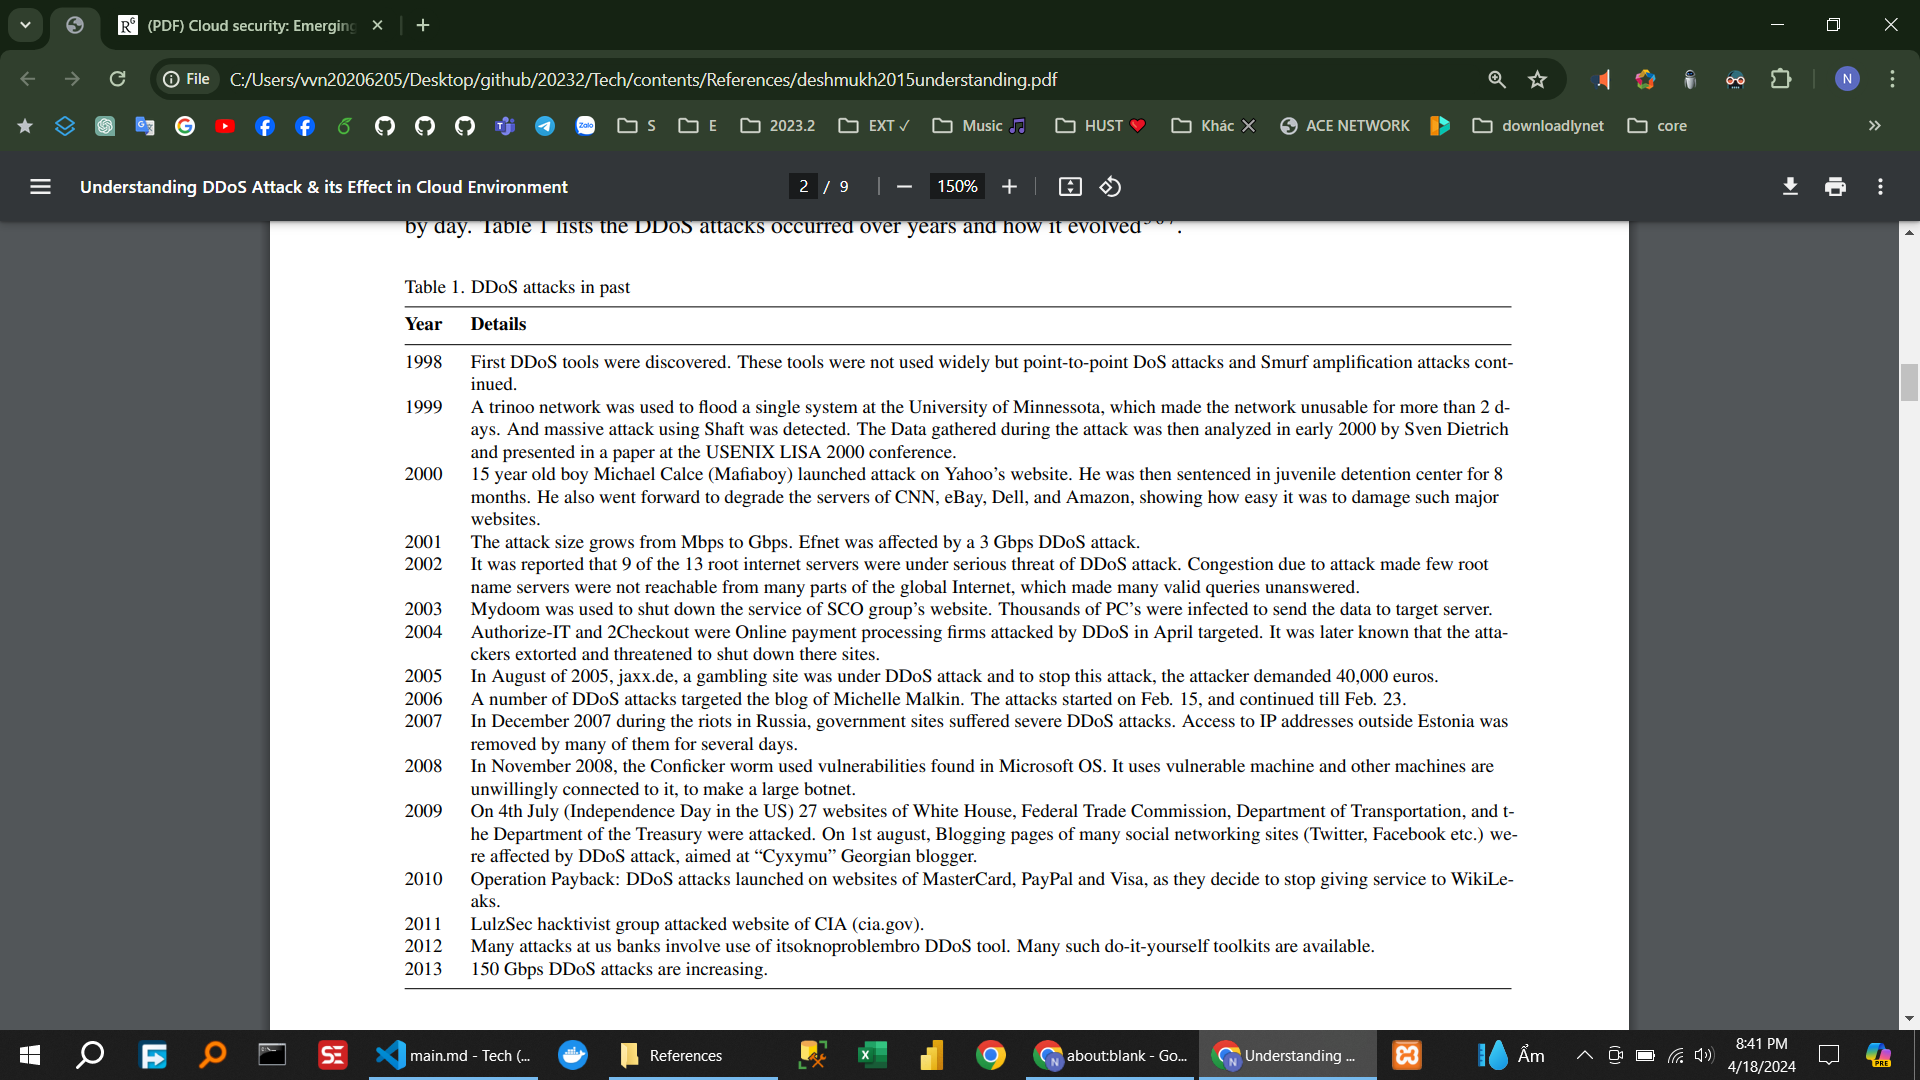
\includegraphics[scale = 0.5]{DDoS.png}
\caption{DDoS attacks in past}
\end{figure}
%%%%%%%%%%%%%%%%%%%%%%%%%%%%%%%%%%%%%%%%%%%%%%%%%%%%%%%

\subsubsection{Contribution to Group Work}
\begin{itemize}
\item Support for "Distributed Denial-of-Service (DDoS) Attack" section
\end{itemize}
%%%%%%%%%%%%%%%%%%%%%%%%%%%%%%%%%%%%%%%%%%%%%%%%%%%%%%%
\subsection{Paper Title: "A Survey of Security and Privacy Challenges in Cloud Computing: Solutions and Future Directions" \cite{liu2015survey}}

\subsubsection{Main Contribution}
In the "SECURITY AND PRIVACY CHALLENGES" section, there is a summary as follows:
\begin{itemize}
\item Loss of Control: Users experience diminished control over their data when moving from local servers to remote cloud servers.
\item Data Breaches: Data loss and breaches are recognized as top threats in cloud computing environments.
\item Multi-Region Regulations: Data may be stored across data centers in multiple legal jurisdictions, raising concerns about compliance with local laws.
\item Managerial Challenges: Non-technical managerial issues are closely related to technical solutions needed to address corresponding technical challenges.
\end{itemize}

\subsubsection{Personal Judgement}
\begin{itemize}
\item Security and privacy issues in the cloud computing environment are truly a significant challenge. Attacks and data breaches are also serious threats, especially when data stored in multiple locations can be affected. This poses a challenge for businesses and organizations when deploying and managing cloud computing environments.
\end{itemize}

\subsubsection{Contribution to Group Work}
\begin{itemize}
\item Support for "Security and Privacy challenges" section
\end{itemize}
%%%%%%%%%%%%%%%%%%%%%%%%%%%%%%%%%%%%%%%%%%%%%%%%%%%%%%%
\subsection{Paper Title: "Cloud security: Emerging threats and current solutions" \cite{coppolino2017cloud}}

\subsubsection{Main Contribution}
In the "Attack Vectors" section, there is a summary as follows:
\begin{itemize}
\item Network: Network-based attacks can impact security, data integrity, and the availability of CP data centers.
\item Hypervisor: Internal users can exploit the hypervisor to attack other VM instances, especially in multi-tenant environments.
\item Hardware: Hardware-based attacks can leverage the multi-tenancy environment to access physical resources like memory, disk buses, and cache.
\item Defense Measures: Discusses defense solutions against network, hardware, and hypervisor-based attacks, including emerging technologies like Intel SGX and ARM TrustZone.
\end{itemize}

\subsubsection{Personal Judgement}
\begin{itemize}
\item These issues underscore the diversity and complexity of threats that a multi-tenant environment may face. Protecting against attacks from various angles necessitates a combination of defensive measures and foresight to address potential threats. Emphasizing emerging technologies such as Intel SGX and ARM TrustZone is also a proactive response, as they can provide additional layers of protection to thwart advanced attacks.
\end{itemize}

\subsubsection{Contribution to Group Work}
\begin{itemize}
\item Support for "Attacking vectors" section
\end{itemize}
%%%%%%%%%%%%%%%%%%%%%%%%%%%%%%%%%%%%%%%%%%%%%%%%%%%%%%%
\newpage
\renewcommand{\refname}{References}
\bibliographystyle{plain}
\bibliography{References}
%%%%%%%%%%%%%%%%%%%%%%%%%%%%%%%%%%%%%%%%%%%%%%%%%%%%%%%
%%%%%%%%%%%%%%%%%%%%%%%%%%%%%%%%%%%%%%%%%%%%%%%%%%%%%%%
%%%%%%%%%%%%%%%%%%%%%%%%%%%%%%%%%%%%%%%%%%%%%%%%%%%%%%%
\end{document}

\begin{figure}[H]
\centering
\includegraphics[scale = 0.15]{xxxxxxxxxxxxxxxxxxxxxxxxxxxxxxxxxxxxxxxx}
\caption{xxxxxxxxxxxxxxxxxxxxxxxxxxxxxxxxxxxxxxxx}
\end{figure}

%%%%%%%%%%%%%%%%%%%%%%%%%%%%%%%%%%%%%%%%%%%%%%%%%%%%%%%
%%%%%%%%%%%%%%%%%%%%%%%%%%%%%%%%%%%%%%%%%%%%%%%%%%%%%%%
%%%%%%%%%%%%%%%%%%%%%%%%%%%%%%%%%%%%%%%%%%%%%%%%%%%%%%%